\documentclass[
	% -- opções da classe memoir --
	12pt,				% tamanho da fonte
	openright,			% capítulos começam em pág ímpar (insere página vazia caso preciso)
	twoside,			% para impressão em verso e anverso. Oposto a oneside
	a4paper,			% tamanho do papel. 
	% -- opções da classe abntex2 --
	%chapter=TITLE,		% títulos de capítulos convertidos em letras maiúsculas
	%section=TITLE,		% títulos de seções convertidos em letras maiúsculas
	%subsection=TITLE,	% títulos de subseções convertidos em letras maiúsculas
	%subsubsection=TITLE,% títulos de subsubseções convertidos em letras maiúsculas
	% -- opções do pacote babel --
	english,			% idioma adicional para hifenização
	french,				% idioma adicional para hifenização
	spanish,			% idioma adicional para hifenização
	brazil				% o último idioma é o principal do documento
	]{abntex2}

% ---
% Pacotes básicos 
% ---
\usepackage{pslatex}			% Usa a fonte Latin Modern			
\usepackage[T1]{fontenc}		% Selecao de codigos de fonte.
\usepackage[utf8]{inputenc}		% Codificacao do documento (conversão automática dos acentos)
\usepackage{lastpage}			% Usado pela Ficha catalográfica
\usepackage{indentfirst}		% Indenta o primeiro parágrafo de cada seção.
\usepackage{color}				% Controle das cores
\usepackage{graphicx}			% Inclusão de gráficos
\usepackage{microtype} 			% para melhorias de justificação
% ---
		
% ---
% Pacotes adicionais, usados apenas no âmbito do Modelo Canônico do abnteX2
% ---
\usepackage{lipsum}				% para geração de dummy text
% ---

% ---
% Pacotes de citações
% ---
\usepackage[brazilian,hyperpageref]{backref}	 % Paginas com as citações na bibl
\usepackage[alf]{abntex2cite}	% Citações padrão ABNT

% --- 
% CONFIGURAÇÕES DE PACOTES
% --- 

% ---
% Configurações do pacote backref
% Usado sem a opção hyperpageref de backref
\renewcommand{\backrefpagesname}{Citado na(s) página(s):~}
% Texto padrão antes do número das páginas
\renewcommand{\backref}{}
% Define os textos da citação
\renewcommand*{\backrefalt}[4]{
	\ifcase #1 %
		Nenhuma citação no texto.%
	\or
		Citado na página #2.%
	\else
		Citado #1 vezes nas páginas #2.%
	\fi}%
% ---

% ---
% Informações de dados para CAPA e FOLHA DE ROSTO
% ---
\titulo{Otimização para motores de busca de um blog: Estudo de caso}
\autor{Jean Miguel Ferreira Dias}
\local{Franca}
\data{2014}
\orientador{Leandro Borges}
\instituicao{%
  Centro Universitário de Franca - Uni-FACEF
  }
\tipotrabalho{Trabalho de Conclusão de Curso}
% O preambulo deve conter o tipo do trabalho, o objetivo, 
% o nome da instituição e a área de concentração 
\preambulo{Trabalho de Conclusão para o curso de Sistemas de Informação}
% ---


% ---
% Configurações de aparência do PDF final

% alterando o aspecto da cor azul
\definecolor{blue}{RGB}{41,5,195}

% informações do PDF
\makeatletter
\hypersetup{
     	%pagebackref=true,
		pdftitle={\@title}, 
		pdfauthor={\@author},
    	pdfsubject={\imprimirpreambulo},
	    pdfcreator={LaTeX with abnTeX2},
		pdfkeywords={abnt}{latex}{abntex}{abntex2}{trabalho acadêmico}, 
		colorlinks=true,       		% false: boxed links; true: colored links
    	linkcolor=blue,          	% color of internal links
    	citecolor=blue,        		% color of links to bibliography
    	filecolor=magenta,      		% color of file links
		urlcolor=blue,
		bookmarksdepth=4
}
\makeatother
% --- 

% --- 
% Espaçamentos entre linhas e parágrafos 
% --- 

% O tamanho do parágrafo é dado por:
\setlength{\parindent}{1.3cm}

% Controle do espaçamento entre um parágrafo e outro:
\setlength{\parskip}{0.2cm}  % tente também \onelineskip

% ---
% compila o indice
% ---
\makeindex
% ---

% ----
% Início do documento
% ----
\begin{document}

% Retira espaço extra obsoleto entre as frases.
\frenchspacing 

% ----------------------------------------------------------
% ELEMENTOS PRÉ-TEXTUAIS
% ----------------------------------------------------------
% \pretextual

% ---
% Capa
% ---
\imprimircapa
% ---

% ---
% Folha de rosto
% (o * indica que haverá a ficha bibliográfica)
% ---
\imprimirfolhaderosto*
% ---

% ---
% Inserir a ficha bibliografica
% ---

% Isto é um exemplo de Ficha Catalográfica, ou ``Dados internacionais de
% catalogação-na-publicação''. Você pode utilizar este modelo como referência. 
% Porém, provavelmente a biblioteca da sua universidade lhe fornecerá um PDF
% com a ficha catalográfica definitiva após a defesa do trabalho. Quando estiver
% com o documento, salve-o como PDF no diretório do seu projeto e substitua todo
% o conteúdo de implementação deste arquivo pelo comando abaixo:
%
% \begin{fichacatalografica}
%     \includepdf{fig_ficha_catalografica.pdf}
% \end{fichacatalografica}
\begin{fichacatalografica}
	\vspace*{\fill}					% Posição vertical
	\hrule							% Linha horizontal
	\begin{center}					% Minipage Centralizado
	\begin{minipage}[c]{12.5cm}		% Largura
	
	\imprimirautor
	
	\hspace{0.5cm} \imprimirtitulo  / \imprimirautor. --
	\imprimirlocal, \imprimirdata-
	
	\hspace{0.5cm} \pageref{LastPage} p. : il. (algumas color.) ; 30 cm.\\
	
	\hspace{0.5cm} \imprimirorientadorRotulo~\imprimirorientador\\
	
	\hspace{0.5cm}
	\parbox[t]{\textwidth}{\imprimirtipotrabalho~--~\imprimirinstituicao,
	\imprimirdata.}\\
	
	\hspace{0.5cm}
		1. Palavra-chave1.
		2. Palavra-chave2.
		I. Orientador.
		II. Universidade xxx.
		III. Faculdade de xxx.
		IV. Título\\ 			
	
	\hspace{8.75cm} CDU 02:141:005.7\\
	
	\end{minipage}
	\end{center}
	\hrule
\end{fichacatalografica}
% ---

% ---
% Inserir folha de aprovação
% ---

% Isto é um exemplo de Folha de aprovação, elemento obrigatório da NBR
% 14724/2011 (seção 4.2.1.3). Você pode utilizar este modelo até a aprovação
% do trabalho. Após isso, substitua todo o conteúdo deste arquivo por uma
% imagem da página assinada pela banca com o comando abaixo:
%
% \includepdf{folhadeaprovacao_final.pdf}
%
\begin{folhadeaprovacao}

  \begin{center}
    {\ABNTEXchapterfont\large\imprimirautor}

    \vspace*{\fill}\vspace*{\fill}
    \begin{center}
      \ABNTEXchapterfont\bfseries\Large\imprimirtitulo
    \end{center}
    \vspace*{\fill}
    
    \hspace{.45\textwidth}
    \begin{minipage}{.5\textwidth}
        \imprimirpreambulo
    \end{minipage}%
    \vspace*{\fill}
   \end{center}
        
   Trabalho aprovado. \imprimirlocal, 24 de novembro de 2012:

   \assinatura{\textbf{\imprimirorientador} \\ Orientador} 
   \assinatura{\textbf{Professor} \\ Convidado 1}
   \assinatura{\textbf{Professor} \\ Convidado 2}
   %\assinatura{\textbf{Professor} \\ Convidado 3}
   %\assinatura{\textbf{Professor} \\ Convidado 4}
      
   \begin{center}
    \vspace*{0.5cm}
    {\large\imprimirlocal}
    \par
    {\large\imprimirdata}
    \vspace*{1cm}
  \end{center}
  
\end{folhadeaprovacao}
% ---

% ---
% Dedicatória
% ---
\begin{dedicatoria}
   \vspace*{\fill}
   \centering
   \noindent
   \textit{ Este trabalho é dedicado aos corajosos e persistentes que buscam\\ aumentar as visitas em seus blogs e websites.} \vspace*{\fill}
\end{dedicatoria}
% ---

% ---
% Agradecimentos
% ---
\begin{agradecimentos}
Os agradecimentos principais são direcionados à Gerald Weber, Miguel Frasson,
Leslie H. Watter, Bruno Parente Lima, Flávio de Vasconcellos Corrêa, Otavio Real
Salvador, Renato Machnievscz\footnote{Os nomes dos integrantes do primeiro
projeto abn\TeX\ foram extraídos de
\url{http://codigolivre.org.br/projects/abntex/}} e todos aqueles que
contribuíram para que a produção de trabalhos acadêmicos conforme
as normas ABNT com \LaTeX\ fosse possível.

Agradecimentos especiais são direcionados ao Centro de Pesquisa em Arquitetura
da Informação\footnote{\url{http://www.cpai.unb.br/}} da Universidade de
Brasília (CPAI), ao grupo de usuários
\emph{latex-br}\footnote{\url{http://groups.google.com/group/latex-br}} e aos
novos voluntários do grupo
\emph{\abnTeX}\footnote{\url{http://groups.google.com/group/abntex2} e
\url{http://abntex2.googlecode.com/}}~que contribuíram e que ainda
contribuirão para a evolução do \abnTeX.

\end{agradecimentos}
% ---

% ---
% Epígrafe
% ---
\begin{epigrafe}
    \vspace*{\fill}
	\begin{flushright}
		\textit{``Não vos amoldeis às estruturas deste mundo, \\
		mas transformai-vos pela renovação da mente, \\
		a fim de distinguir qual é a vontade de Deus: \\
		o que é bom, o que Lhe é agradável, o que é perfeito.\\
		(Bíblia Sagrada, Romanos 12, 2)}
	\end{flushright}
\end{epigrafe}
% ---

% ---
% RESUMOS
% ---

% resumo em português
\setlength{\absparsep}{18pt} % ajusta o espaçamento dos parágrafos do resumo
\begin{resumo}
 Segundo a \citeonline[3.1-3.2]{NBR6028:2003}, o resumo deve ressaltar o
 objetivo, o método, os resultados e as conclusões do documento. A ordem e a extensão
 destes itens dependem do tipo de resumo (informativo ou indicativo) e do
 tratamento que cada item recebe no documento original. O resumo deve ser
 precedido da referência do documento, com exceção do resumo inserido no
 próprio documento. (\ldots) As palavras-chave devem figurar logo abaixo do
 resumo, antecedidas da expressão Palavras-chave:, separadas entre si por
 ponto e finalizadas também por ponto.

 \textbf{Palavras-chaves}: latex. abntex. editoração de texto.
\end{resumo}

% resumo em inglês
\begin{resumo}[Abstract]
 \begin{otherlanguage*}{english}
   This is the english abstract.

   \vspace{\onelineskip}
 
   \noindent 
   \textbf{Key-words}: latex. abntex. text editoration.
 \end{otherlanguage*}
\end{resumo}

% ---
% inserir lista de ilustrações
% ---
\pdfbookmark[0]{\listfigurename}{lof}
\listoffigures*
\cleardoublepage
% ---

% ---
% inserir lista de tabelas
% ---
\pdfbookmark[0]{\listtablename}{lot}
\listoftables*
\cleardoublepage
% ---

% ---
% inserir lista de abreviaturas e siglas
% ---
\begin{siglas}
  \item[SEO] Search Engine Optimiztion
  \item[SEM] Search Engine Marketing
  \item[HTML] Hyper-Text Market Language
  \item[URL] Uniform Resource 
  \item[URI]
\end{siglas}
% ---

% ---
% inserir lista de símbolos
% ---
%\begin{simbolos}
%  \item[$ \Gamma $] Letra grega Gama
%  \item[$ \Lambda $] Lambda
%  \item[$ \zeta $] Letra grega minúscula zeta
%  \item[$ \in $] Pertence
%\end{simbolos}
% ---

% ---
% inserir o sumario
% ---
\pdfbookmark[0]{\contentsname}{toc}
\tableofcontents*
\cleardoublepage
% ---



% ----------------------------------------------------------
% ELEMENTOS TEXTUAIS
% ----------------------------------------------------------
\textual

% ----------------------------------------------------------
% Introdução (exemplo de capítulo sem numeração, mas presente no Sumário)
% ----------------------------------------------------------
\chapter*[Introdução]{Introdução}
\addcontentsline{toc}{chapter}{Introdução}
% ----------------------------------------------------------

SEO é um sigla que significa Search Engine Optimization na tradução Otimização para Motores de Busca, que se refere a uma técnica responsável por fazer um website alcançar melhor visibilidade nas buscas, em ferramentas como o Google, Bing, Yahoo, entre outros. 

Jerkovic (2009) define SEO como um agregado de todo o trabalho necessário para produzir um alto volume de referências bem-sucedidas oriundas de mecanismos de busca, diretórios web e outros websites, com o objetivo final de popularizar o website.

As técnicas usadas para melhorar o posicionamento de um website dentro dos grandes buscadores são várias, desde análises internas e externas do website, trabalho com mídias sociais, criação de links em sites de terceiros, otimizar conteúdo para palavras-chaves, criação de conteúdo e outras tarefas.

Mas antes de aprofundar em no tema do SEO precisamos entender alguns conceitos que servem como base para conseguir melhor consciência para implantar as técnicas de otimização em seu website. Com isso, para entender qual o motivo de otimizar um website, e quais fatores deve ser levados em consideração, é necessário entender os conceitos básicos do SEO. 


% ----------------------------------------------------------
% PARTE
% ----------------------------------------------------------
% \part{Referenciais teóricos}
% ----------------------------------------------------------

% ---
% Capitulo de revisão de literatura
% ---

\chapter{Otimização para Mecanismos de Busca}

\section{Motores de Busca}

Os motores de busca surgiram logo após a criação da Internet como conhecemos hoje. Segundo Ledford (2008) a primeira ferramenta de busca foi lançado em 1990, chamado Archie. A necessidade de se criar ferramentas que possibilitassem efetuar buscas dentro da Internet apareceu por causa da complexidade que era encontrar arquivos ou textos dentro da web.

A forma em que era encontrado um texto ou arquivos no começo da Internet não era nada parecido com o que nós temos hoje. Para você ter acesso a algo, a Internet baseava-se em um conjunto de pastas organizadas e para se ter acesso era necessário ter acesso por um protocolo de rede chamado de FTP (File Transfer Protocol, em português Protocolo de Transferência de Arquivos), onde permitia que aos usuários obter o acesso a estas pastas e procurar os arquivos que lhe sejam uteis.

Encontrar algo desta forma era bastante trabalhoso, pois consistia do usuário ter que navegar de pasta em pasta para achar a arquivo que o mesmo procurava. É lógico que existiam atalhos que levava o usuário até o seu destino rapidamente, mas era necessário saber onde encontrar estes atalhos, geralmente fornecidos quando você já sabia qual o arquivo exato você está procurando.

Com isso o processo para encontrar um arquivo na Internet para Ledford (2008) na prática, era um exercício difícil e demorado de paciência. Contudo em 1990 o estudante da universidade de McGill, em Montreal – Canadá, Alan Emtange criou a primeira ferramenta, que se tem registro, para busca na Internet chamada Archie, que era um índice com os arquivos da Internet.

A forma em que este programa denominado como Archie trabalhava está muito distante de como funciona os mecanismos de busca hoje em dia. Pois seu trabalho consistia em baixar um lista de todos os arquivos dentro daquela pasta na Internet, e está lista era baixada para dentro de um banco de dados de websites, podendo assim ser consultado disponibilizando a informação de um forma mais rápida.

O Archie servia apenas para listar arquivos de um FTP, não para procurar por arquivos relacionados a termo de busca, como acontece com os buscadores atualmente. Em 1991 outro estudante Mark McCahill da Universidade de Minnesota, percebeu que se existia a possibilidade de indexar arquivos, que era o que o Archie fazia, também era possível fazer busca de textos puro em referência de arquivos.

A partir disso como não existia nenhum aplicativo que realizava essa tarefa, ele criou o Gopher, um programa que permite indexar arquivos em texto puro, na figura 1.1 é possível ver como era o índice do programa, que segundo Ledford (2008) veio a se tornar os primeiros websites da Internet pública. Com isso a forma com que realmente funciona as buscas atualmente começou a amadurecer.

\begin{figure}[hbtp]
\caption{Índice do Gopher}
\centering
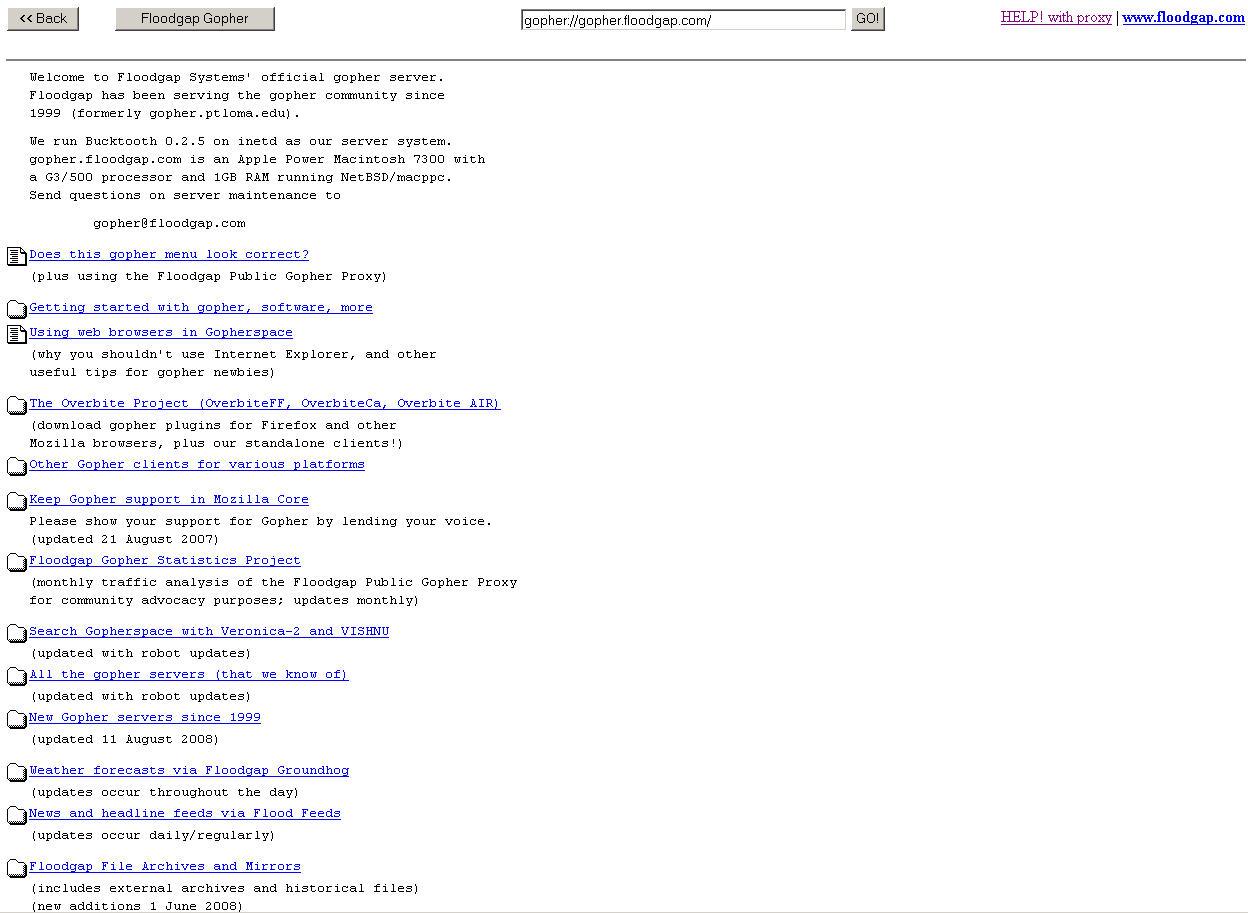
\includegraphics[totalheight=0.5\textheight]{img/indice-gopher.png}
\label{who}
\legend{Fonte: Wikipedia, 2008}
\end{figure}

Mas para o Gopher funcionar com da maneira esperada foi necessária a criação de duas novas aplicações a Veronica (Very Easy Easy Rodent-Oriented Net-wide Index to Computerized, na tradução Índice Bastante Fácil para Arquivos Computadorizados em Rede) e Jughead (Jonzy’s Universal Gopher Hierarchy Excavation and Display, na tradução Escavação e Exibição Universal da Hierarquia do Gopher por Jonzy) que serviam para procurar os arquivos indexados nos índices do Gopher, denominado de Gopher Index System (na tradução Sistema de Índices do Gopher).

Mas só em 1993 desenvolvido por Matthew Gray aplicação denominada de Wandex, foi o primeiro programa a fazer tanto a indexação como também a busca nos índice da páginas da web. Segundo Ledford (2008) essa tecnologia foi o primeiro programa a vascular a web, e posteriormente se tornou a base para todos os crawlers de busca. No período de 1993 até o início do século 2000, foram desenvolvidos basicamente todos os motores de busca mais conhecidos do mercado, como o Yahoo em 1994, Google em 1997 e o MSN Search em 1998 que veio a se chamar Bing em 2008.

Estes três mecanismos de busca, Google, Yahoo e Bing são os mais populares do mercado na parte ocidental do globo, sendo o Google criado por Larry Page e Sergey Brin na Universidade de Stanford, em pesquisa feita pela comScore \url{http://goo.gl/IkS0uZ} em Março de 2014 nos Estados Unido, ele ocupa 67,5\% das preferências de busca, seguido pelo Bing com 18,6\%, Yahoo com 10,1\% e outros com 3,8\%.

Dentro deste mercado de motores de busca Jerkovic (2009) separa os mecanismos de buscas em alguns grupos, que são: motores de busca de primários, mecanismos de busca secundários, mecanismos de busca regionais, motores de busca verticais, mecanismos baseados em web spiders, motores de busca híbridos e baseados em metabusca.

\section{Funcionamento de um Motor de Busca}

No ponto de vista de um usuário final o motor de busca é apenas um simples website, que quando você precisa de procurar por algum termo na web você simplesmente digite essa palavra ou expressão em um campo, e a seguir pressiona a tecla “Enter” ou clica em pesquisar, onde que a partir destes pequenos passos vão surgir milhares de respostas para aquele termo digitado.

Mas essa definição fica por parte de um usuário final que não compreende realmente o que está acontecendo no back end do motor de busca. Vamos dividir o motor de busca em duas partes o back end e o front end, onde que no back end do motor contém a parte responsável por tudo funcionar e as buscas retornarem resultados, e o front end do motor apenas fica responsável por exibir para o usuário final estes resultados.

O back end de um motor de busca é apenas um software que segundo Ledford (2008) utiliza-se de aplicativos para coletar informações sobre páginas web. Estes aplicativos são chamados de crawlers, spiders ou robôs web. Ledford (2008) classifica estas informações coletadas como: palavras-chaves, expressões que represente o conteúdo da página web como um todo, a URL da página, e a estrutura dos links que saem e entram na página.

Com isso o motor de busca armazena estas informações a respeito de uma página web em um banco de dados. No front end que é a página web onde o usuário final digita seu termo para busca, o motor executa as seguintes tarefas: o motor irá pegar este termo digitado, ele fará uma consulta no banco de dados procurando se existe alguma página da web que contém aquele termo e após isso retornará todos os resultados encontrados exibindo-os ao usuário que efetuou a busca.

\section{Tipos de Mecanismos}

\subsection{Mecanismos Primários}

Para Jerkovic (2009) Bing, Google e Yahoo são mecanismos de busca primários, pois os três motores detêm maior fatia do mercado de pesquisas do mundo. Nesses tipos de mecanismo funcionam de forma que eles vasculham todas as páginas da Internet criando enormes banco de dados de índices, utilizados nas buscas.

Estes mecanismos de buscas primários são capazes de indexar a maioria ou até todos os websites da Internet, onde que Ledford (2008) fala que a diferença no resultados deles fica apenas por conta de como o algoritmo do motor funciona, isto faz com que o mesmo termo procurado em um motor resulte em diferentes resultados em outro.

\subsection{Mecanismos Secundários}

Os mecanismos de busca secundários não tem o mesmo volume de acessos de um mecanismos principais pois geralmente são voltados para públicos mais específicos, isso faz com que o número de usuários que utilizam um mecanismo de busca primário seja maior que o motores de busca secundários.

No entanto mesmo Jerkovic (2009) apresentar que estes mecanismos são menos renomados e não tão populares quanto um mecanismo de busca primário, Ledford (2008) defende falando que para buscas regionais ou mais focadas eles podem ser bastante uteis. Motores de buscas secundário podem ser citados como: Lycos, Ask, LookSmart, entre outros. 

\subsection{Mecanismos Regionais}

Mesmo os mecanismos de buscas primários seja os quem geram maior trafego na Internet, existem os mecanismos regionais que são motores mais específicos para buscas em determinadas regiões, como o Baidu na China, que quando você utiliza-lo seus resultados de busca são mais focados em páginas da Internet daquela região.

\subsection{Mecanismos Vericais}

Jerkovic (2009) chama-os de mecanismos de busca especializados, pelo fato de que os motores de buscas verticais pesquisam resultados mais específicos de um único tema, por exemplo um mecanismo de busca que contém apenas resultados para um único tópico como esportes, arte, ciências, literatura entre outros.
Mecanismos baseados em web spiders

Para Jerkovic (2009) os mecanismos de busca baseados em web spiders são definos assim:


\begin{citacao}
Mecanismos de busca baseados em web spiders usam programas, o web spider, para criar seus índices de bancos de dados. Além do Google, Yahoo! e Microsoft, essa classe de mecanismo de busca inclui:

\item Cuil (http://www.cuil.com)
\item Exalead (http://www.exalead.com)
\item Gigablast (http://www.gigablast.com)
\item Teoma/Ask (http://www.ask.com)
\item Walhello (http://www.walhello.com)
\cite[5.3]{NBR10520:2002}.
\end{citacao}

\subsection{Mecanismos Hibridos}

No mercado atual de buscas alguns mecanismos apresentam várias formas de efetuar pesquisa, por diversas categorias diferentes tal como ocorre nos motores de busca vertical. Estes mecanismo de busca são classificados como mecanismos de busca híbridos, que segundo Jerkovic (2009) é a unificação de uma variedade de resultados, onde é possível incluir resultados de spiders, diretórios web, notícias, produtos entre outros.

Motores de busca como Bing, Google e Yahoo! já adotaram este modelo de busca, que Jerkovic (2009) denomina de Busca Universal, onde que a ideias basicamente e informar múltiplos resultados para um termo, tornando assim a busca mais rica e completa. Na figura 1.2 é possível ver estes detalhes.

Na figura 1.2 é possível perceber como funciona um motor de busca hibrido, pelo fato da busca ser pela palavra “carro” é possível perceber que o mecanismo de busca retorna vários resultados diferentes, como os links de publicidade, uma área onde se encontra imagens sobre o termo procurado.

\begin{figure}[hbtp]
\caption{Resultados Variados do Bing}
\centering
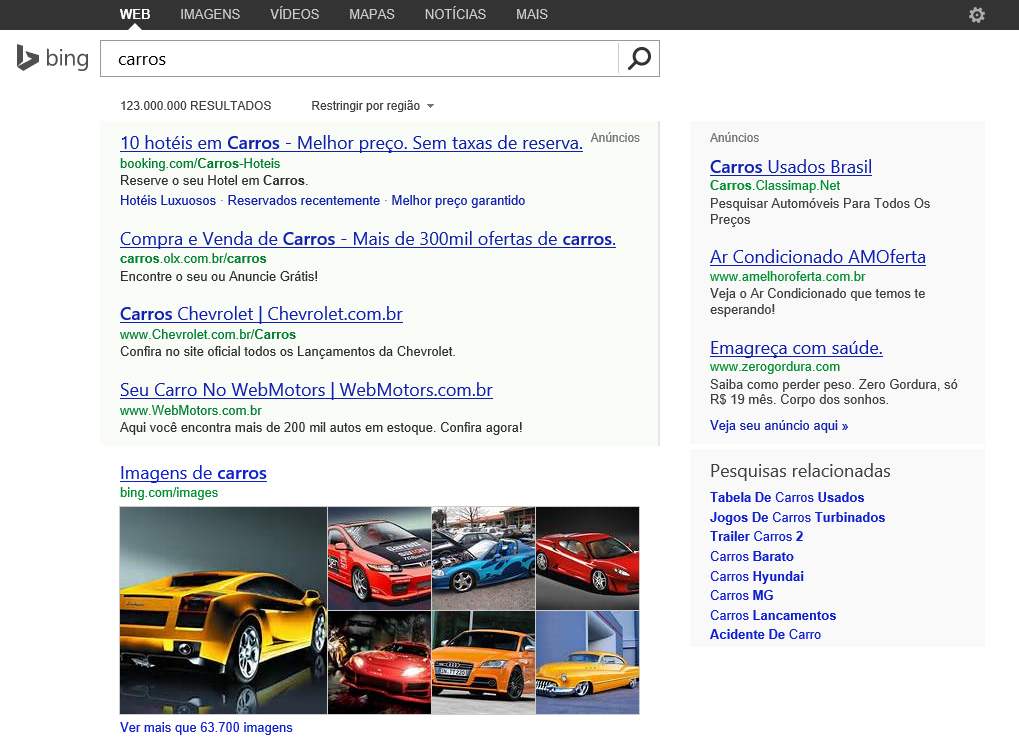
\includegraphics[totalheight=0.5\textheight]{img/resultados-bing.jpg}
\label{who}
\legend{Fonte: o Autor}
\end{figure}

\subsection{Mecanismos Metabusca}

Jerkovic (2009) cita que se o usuário buscar pelo mesmo termo em diferentes mecanismos de buscas a base de spiders, eles lhe retornaram resultados diferentes, que ao contrário dos motores baseados em metabusca é organizar e juntar resultados de vários motores, fazendo com que assim aumente a qualidade nos resultados retornados.

\section{Rôbos}

Os aplicativos responsáveis por alimentar o banco de dados de um motor de busca são conhecidos como Spiders, Crawlers ou Robôs Web, que tem como tarefa básica percorrer por todas as páginas web procurando por pelas informações que são armazenadas no banco de dados do motor de busca, Ledford (p7, 2008) explica o que são estes três programas da seguinte forma:

\begin{citacao}
Essas pequenas criaturas são programas que literalmente vasculham a web, catalogando dados para que estes possam ser buscas pelos usuários. No sentido mais básico, todos os três programas – crawlers, spiders e robôs – são essencialmente a mesma coisa. Todos eles coletam informações sobre todas as URLs da web.
\cite[p7]{NBR10520:2002}.
\end{citacao}

Com isso todas estas informações coletadas por estes três programas são catalogadas de acordo com sua URL (Uniform Resource Locator, na tradução Localizador Padrão de Recursos) para que assim possa ser encontrada após uma busca executada pelo usuário.

Jerkovic (2009) diz que o termo spider, robô e crawler representam a mesma coisa, no qual são aplicativos automatizados que tem como proposito de navegar pela Internet no objetivo de encontrar e fornecer ao seu mecanismo de busca o maior número de websites. Portanto nas próximas vezes que o texto se referir a spiders estará fazendo referência aos três de uma vez só.

Os Spiders atuam de forma aleatória dentro da web, eles navegam pelos websites rastreando não só os links mas também qualquer outro tipo de documento, como arquivos de imagens e vídeos. O acesso dos spiders aos websites podem ser várias vezes ou raramente, que segundo Jerkovic (2009) acontece a partir do tamanho do conteúdo do website.
 
Mas Jerkovic (2009) afirma também que os spiders não irão visitar seu website uma única vez, pois a partir do momento que um spider rastrear a página de seu website ele irá sempre voltar para detectar alterações, adições e exclusões dentro do conteúdo ou da página.

Os spiders de acordo com Ledford (2008) trabalham da seguinte forma: quando eles são lançados na web, eles recebem uma lista de websites que são o ponto de partida para os spiders, e a partir deste momento ele saem rastreando as páginas e encontrando novos links para percorrer.

Estes links que os spiders encontram podem ao mesmo tempo leva-los a outras páginas do mesmo website, como também podem leva-lo completamente para fora deste website. Com isso ele segue este processo até encontrar uma página do website que não leve para lugar nenhum, a partir deste ponto ele recomeça o processo até que todos os links sejam mapeados, segundo Ledford (2008). 

\chapter{Tipos de Busca}

Dentro do cenário de SEO, muitos profissionais se confundem ele com o SEM (Marketing nos mecanismos de Busca) que são os anúncios de “pay-per-click” (Pague pelo Clique, PPC), por exemplo o Google AdWords. Embora ambos tenha alguns elementos em comum, como o foco em palavras-chaves, as implementações de SEM são bem mais simples, e alcançam resultados praticamente de forma imediata, pelo fato de serem formas de campanhas pagas, o SEO para Jerkovic (2009) é a forma mais próxima de uma propaganda gratuita que se pode chegar, pois estas técnicas lhe permitem aumentar sua visibilidade de forma natural, não necessitando pagar para aparecer como a primeira opção.

Mas entretanto não se pode dizer que para fazer SEO em um website não precisará desembolsar algum valor inicial, pelo fato do website estar posicionado nas buscas orgânicas, onde ao contrário do PPC, não necessita pagar para estar naquela posição. Fazer SEO exige que se faça investimentos, e seus resultados serão alcançados a longo prazo.

Jerkovic (2009) apresenta a seguinte tabela apontando as vantagens e desvantagens entre SEO ou PCC:

% tabela 1.1

\begin{table}[htb]
\ABNTEXfontereduzida
\caption[Vantagens e Desvantagens SEO x PPC]{Vantagens e Desvantagens SEO x PPC}
\label{tab-nivinv}
\begin{center}
\begin{tabular}{p{2.6cm}|p{6.0cm}|p{2.25cm}|p{3.40cm}}
  %\hline
   \textbf{SEO} \\
   \textbf{Vantagens} & \textbf{Desvantagens} \\
    \hline
    Benefícios a longo prazo & Resultados iniciais demoram \\
    \hline
    Aumenta a credibilidade pelo visitante & Para alguns casos não há garantias \\
   \textbf{PPC} \\
   \textbf{Vantagens} & \textbf{Desvantagens} \\
    \hline
    Tráfego instantâneo & Gasta recursos rapidamente \\
    \hline
    Facilidade de implementação & As melhores posições são para quem paga mais \\
    \hline
    Facilidade de administração & Desconfiança \\
    \hline
    Menor investimento para manutenção & Visitantes param quando para o investimento \\
   % \hline
\end{tabular}
\end{center}
\legend{Fonte: Guerreiro SEO}
\end{table}

Com estes itens começa a perceber quais os grandes desafios dentro do SEO que podem ser elencados como a concorrência, falta de garantias, alterações constantes no ranking e fatores relacionados a tempo.

No mercado para cada setor você encontrará uma serie de competidores, onde que sua empresa, para obter um destaque ao olhos do consumidor necessita mostrar algum diferencial. No mundo virtual funciona da mesma forma existem vários concorrentes no mesmo segmento. Em pesquisa feita pela NetCraft em Abril de 2014, indica que existem 958 milhões de websites, 34 milhões a mais que no mês de março \url{http://goo.gl/zLvFD}.

De acordo com a ONU (Organização das Nações Unidas), em junho de 2013 a população mundial era de 7,2 bilhões, estes dados é possível afirmar que existe aproximadamente um website para cada sete pessoas \url{http://goo.gl/dcCDn6}.

Mas dentro de SEO segundo Jerkovic (2009) ninguém pode verdadeiramente garantir o primeiro lugar no Google, Yahoo! ou Bing. Pois para alcançar um bom ranqueamento dentro deste grandes buscadores, envolve vários aspectos que definem que seu website esteja em posições relevantes. Mas se você aplica todas as estratégias do SEO, tendo um conteúdo de qualidade, melhores posições e popularidade virão com o tempo.

Um outro ponto que afeta o posicionamento de seu website nos mecanismos de busca, fica por conta dos milhares domínios que estão competindo em busca de maior relevância, com isso ganha-se um aumento grande em sua concorrência. Por este motivo os buscadores vivem em constante melhoria para sempre estar retornando resultados relevantes em suas pesquisas.

Mas esse é um fator contempla dois lados, que é possível dizer que existe fatores positivos que auxiliam seu website a ganhar posições e melhorar dentro das buscas, e fatores negativos que servem apenas para atrapalhar seu website fazendo com que ele perda posições em páginas ou nem apareça nos resultados.

Um outro ponto que influencia no SEO é a questão do tempo, pois aplicar essas práticas e conceitos que melhora sua relevância, não é uma tarefa que lhe resultara em retorno a curto prazo. Ele lhe proporciona resultados a longo prazo e de forma natural. Isto faz com que em algum momento seu website comece a receber visitantes a partir de outros buscadores, além de outros websites que estarão vinculados ao seu. 

\section{Busca Organica}

Busca Organica é toda aquela área dos resultados, que aparecem naturalmente.

\section{Busca Paga}

Busca Paga é toda aquela área dos resultados, quem aparecem pelo fato de algum estar patrocinando aquela busca.


\chapter{Processos para Otimização de um Website}

\section{Corpo da Página}

Corpo da página se define pela organização de tags de HTML, atributos de uma tag tais como o title ou alt. Além da adição de tags para melhorar em redes sóciais e também atributos do Schema.org.

\section{Links Internos e Externos}

Links Building

\section{Conteúdo}

Textos de qualidade para as páginas

\section{Ferramentas de Analise}

Visando sempre aprimorar o posicionamento de seu website, fazendo com que ele sempre esteja legível para o Google e além disso possa acompanhar uma análise detalhada para que seja possível avaliar os pontos fortes e pontos fracos de seu website, a própria Google desenvolveu duas ferramentas que são de extrema importância para o administrador do website possa ter informações e estatísticas, o que permitirá a tomada de decisão para gerar mais visitantes.

Essas ferramentas são conhecidas com Google Webmaster Tools e Google Analytics. A primeira ferramenta segundo Jerkovik (2009) permite aos websmaster um meio fácil de rastrear o tráfego de suas páginas, também analisar o arquivo robots.txt, adicionar seus arquivos sitemaps e assim por diante. E a segunda ferramenta o Google Analytics segundo Jerkovic (2009) é a ferramenta de marketing preferida para a visualização de estatísticas web gerais e o mais importante, o acompanhamento de conversões.

Para utilizar ambas as ferramentas é necessário possuir um conta da Google para que assim possa ter acesso ao Google Webmaster Tools e o Google Analytics. Ambas as ferramentas para que possam funcionar de acordo dentro do website e começem a capturar as informações do website para assim exibir para analise, elas precisam primeiro reconhecer o website, tarefa no qual pode ser feita tanto subindo um arquivo com o nome gerado randomicamente pelo Google na raiz do website, como também apartir de uma inserção de código nas páginas do website.

\subsection{Ferramenta para o administrador do website}

O Google Webmaster Tools é uma ferramenta onde é possível administrar vários websites, com isso em sua tela principal aparece uma lista com todos os websites que você administra. No painel esquerdo da ferramenta a partir do momento em que se é selecionado um website, é apresentado um menu com acesso a todas as ferramentas para administração e analise de seu website. Na tabela 2.1 é apresentado uma lista com todas as ferramentas disponíveis no Google Webmaster Tools.

\begin{table}[htb]
\ABNTEXfontereduzida
\caption[Ferramentas do Google Webmaster Tools]{Ferramentas do Google Webmaster Tools}
\label{tab-nivinv}
\begin{center}
\begin{tabular}{p{2.6cm}|p{6.0cm}|p{2.25cm}|p{3.40cm}}
  %\hline
   \textbf{Ferramenta} & \textbf{Descrição} \\
    \hline
    Painel do Site & Mostra uma visão geral do website \\
    \hline
    Mensagens do site & Mostra todas as notificações ou alertas do website \\
    \hline
    Dados estruturados & Mostra uma visão geral se o Google identificou dados estruturados no website \\
    \hline
    Marcador de dados & Permite que você marque os dados estruturados no website \\
    \hline
    Melhorias de HTML & Informa setores do website qe podem ser otimizados \\
    \hline
    Links para o site & Permite rebaixar os sitelinks do website \\
    \hline
    Consutas de pesquisa & Permite visualizar quais são as pesquisas que os usários fazem e acessam o website \\
    \hline
    Links para seu site & Permite visualizar quais são os links de acesso para o website \\
    \hline
    Links internos & Permite visualizar quais os links internos do website \\
    \hline
    Ações manuais & Permite visualizar as ações manuais contra spam no website \\
    \hline
    Segmentação internacional & Permite visualizar para qual publico alvo em nível internacional o website \\
    \hline
    Status do índice & Permite visualizar o status do índice das páginas do website dentro dos resultados do Google \\
    \hline
    Palavras-chave do conteúdo & Permite visualizar quais são as palavras-chaves que aparecem no conteúdo do website \\
    \hline
    Remover URLs & Permite remover URLs do website de dentro dos índices do Google \\
    \hline
    Erros de rastreamento & Exibe todos os erros de rastramento de páginas do website pelo Google \\
    \hline
    Estatísticas de rastreamento & Exibe um relatório de rastreamento do website pelo Googlebot \\
    \hline
    Buscar como o Google & Permite que possa ser procurada páginas no website com o próprio Googlebot \\
    \hline
    Testar robots.txt & Permite que possa ser testado o arquivo robots.txt do website \\
    \hline
    Sitemaps & Permite enviar e verificar quais as URLs do sitemap foram processadas pelo rôbo do Google \\
    \hline
    Parâmetros de URL & Permite adicionar parâmetros para melhor rastreamento das URLs do website \\
    \hline
    Problemas de Segurança & Informa se o website apresenta algum problema relacionado a segurança tal como vunerabilidades \\
    \hline
    Outros recursos & Apresenta sub-ferramentas da própria Google para auxiliar nas melhorias e divulgação do website \\
   % \hline
\end{tabular}
\end{center}
\legend{Fonte: o Autor}
\end{table}

No menu Painel do site na ferramenta Google Webmaster Tools ela apresenta alguns informações mais importantes para analise do website como,  informações de status de rastreamento do website, consulta de pesquisas, sitemap e algumas mensagens críticas. Todos estes dados de forma generica mostrando as informações de uma forma simples sem todos os detalhes que são apresentados em seus respectivos menus.

Na seção Mensegens do site é apresentada todas as mensagens de erros, alertas e notificação sobre o website, onde que o próprio rôbo de busca do Google, o Googlebot, vai identificando em seu rastreio e armazenando e relatando neste painel, para que o webmaster fique informado sobre as situações do website e posso sempre estar corrigindo e melhorando.

A ferramenta de Dados estruturados segundo o Google (2014a) mostra ao websmaster informações estruturadas que o Google detectou em seu site, esta ferramenta permite que o Google analise o website e consiga encontrar as marcações de dados estruturados, o que faz o website ser melhor compreendido pelo motor de busca, e em pesquisas efetivadas pelo usuário o Google possa retornar os seus resultados com melhor precisão.

Na ferramenta Marcador dados é possível selecionar e marcar todas as seções e itens do seu website, para que o Google no momento em que for percorrer pelo website dentro de seu índice, ele automaticamente irá reconhecer as marcações realizadas com o uso da ferramenta, e apresentará o website de uma forma mais agradável exibindo mais itens e informação no resultado.

Melhorias de HTML é  uma ferramenta que permite visualizar problemas encontrados pelo Google durante o rasteamento e a indexação do website. O Google recomenda que seja acessado este painel para identificar os problemas que se forem corrigidos auxilia a aumentar a classificação do website nas páginas de resultados. Segundo o Google (2014b) estas questões não evitam que o site seja rastreado ou indexado, mas cuidar delas permite que o website possa oferecer maior experiência ao usuário e também ajudar a direcionar tráfego ao website.

Entre os dados contidos nas melhorias de HTML o webmaster encontrará informações como: problemas com os títulos das páginas, por exemplo títulos repetidos nas páginas, problemas com a tag meta descrição, podendo ela estar vázia ou duplicada em outras páginas, e até páginas com conteúdo que não pode ser indexado como arquivos de formatos desconhecidos pelo robô de busca.

Na ferramenta Links para o site é permitido que o webmaster possa rebaixar os links para o site que não seja interessante para o usuário, no caso esses links segundo o Google (2014c) são chamados de sitelinks, que tem a finalidade de ajudar o usuário a navegar pelo website com maior facilidade.

Estes sitelinks são exatamente os links exibidos abaixo do link retornado pela busca, na figura 2.1 é exibido no item 1 o link principal do website e no item 2 os sitelinks. Os sitelinks exibidos pelo Google apenas são apresentados caso a estrutura do website permitir, caso eles não sejam pertinentes a consulta do usuário eles nem serão exibidos. Segundo o Google (2014c) ele identifica os sitelinks a partir do texto âncora e atributo alt dos links internos do website.

\begin{figure}[hbtp]
\caption{Webmaster sitelinks}
\centering
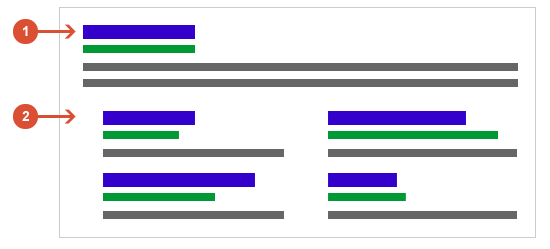
\includegraphics[totalheight=0.3\textheight]{img/webmaster-sitelinks.png}
\label{who}
\legend{Fonte: Google, 2014c}
\end{figure}

Consultas de pesquisa é a página dentro do Google Webmaster Tools em que é possível visualizar as consultas efetuadas no Google, em que as mesma retornam páginas do website, nesta ferramenta é possível ter dados como a taxa cliques (CTR) no website para cada termo procurado, como também a posição média da página dentro dos resultados.

Na ferramenta Links para seu site é a parte do Google Webmaster Tools onde ele classifica todos os links de websites de terceiros que apontam para o website que está sendo gerenciado. Dentro do ferramenta de busca do Google, segundo o mesmo (2014d), ele indica que se for digitado na pesquisa o termo por exemplo "link:tccseo.com.br", a busca retornará páginas da web que aponta para o website.

Na área de Links internos, a ferramenta mostra os links do website que possuem entradas internas para páginas do próprio website, que no caso são sub-links para páginas internas.

Ações manuais é uma página do Google Webmaster Tools que tem como objetivo apresentar ações manuais realizadas pelo próprio Google afim de previnir que em seus resultados apareçam websites que utilizam de técnicas de spam. O Google (2014e) cita que mesmo que seus algoritmos sejam sempre atualizados para previnir isso, ele podem utilizar técnicas manuais para rebaixar ou até mesmo excluir a página dos resultados.

\begin{citacao}
Embora o Google use algoritmos para avaliar e aprimorar regularmente a qualidade da pesquisa, também estamos dispostos a realizar ações manuais em sites que usam técnicas com spam, como rebaixar ou até remover esses sites de nossos resultados de pesquisa completamente.
\cite[p7]{NBR10520:2002}.
\end{citacao}

O Google (2014e) informa que caso seu website ou uma página não apareça mais nos resultados, deve-se consultar a página de Ações manuais para ver os procedimentos necessários para fazer a página voltar, e que ao realizar tais procedimentos é possível solicitar ao Google uma análise diretamente do website ou da página em questão para que ele volte aos resultados.

Na página de Segmentação Internacional para o administrador do website o Google permite que caso o website tenha versões diferentes para cada idioma ou região, é possível tomar medidas para que o conteúdo em específico do website alcance o público-alvo para aquela página. Para fazer isso o Google (2014f) explica que basta adicionar uma tag de HTML no cabeçalho do website para que ele identifique qual a página recomendada para cada região. Na trecho a seguir o Google (2014f) explica três forma para fazer essa marcação.

\begin{citacao}
Para isso, é possível usar três mecanismos de implementação:
\item \textbf{Marcação no nível da página}: Use a tag <link rel='alternate' hreflang='x' href='alternateURL'> na seção <head> das suas páginas para listar as versões alternativas de idioma de cada uma delas. Cada página deve fornecer uma tag hreflang que vincule a todas as suas outras variantes de idioma, assim como uma tag de referência que direcione para a página original. Para uma segmentação mais granular, use o atributo hreflang para indicar as combinações de idioma e país (por exemplo, en-ie, en-ca, en-us). Leia mais sobre a tag hreflang  na seção "Diretrizes de conteúdo".  
\item \textbf{Sitemaps}: Use Sitemaps para enviar opções alternativas de idioma e região para suas páginas. Leia mais sobre o uso de Sitemaps para indicar as páginas com idiomas alternativos na seção "Diretrizes de conteúdo".
\item \textbf{Cabeçalhos HTTP}: Se você publicar arquivos que não sejam HTML, como PDFs, use um cabeçalho HTTP para indicar uma versão em um idioma diferente de um URL.
\end{citacao}

A seção Status do índice dentro do Google Webmaster Tools, segundo o Google (2014g) ela fornece estatísticas sobre os URLs indexados pelo motor do Google para o website em questão.

Palavras-chave de conteúdo é um área da ferramenta do Google que possibilita o administrador do website por visualizar as palavras-chaves que a própria Google identifica dentro do conteúdo do website, com esta informação é possível direcionar o esforços em SEO para algumas palavras-chaves que o Google identifica que sejam mais relevantes no próprio website.

A ferramenta Remover URLs dentro do Google Webmaster Tools é uma ferramenta que permite que o administrador remova determinadas URLs que estejam indexadas pelo Google mas que não sejam necessárias estarem lá. Com isso é possível enviar uma solicitação de exclusão de URLs do index do Google, a própria Google sugere que você especifique no arquivo \textbf{robots.txt} quais seção do website o administrador do mesmo deseja que não seja indexado.

Na página Erros de rastreamento o Google informa ao administrador do website quais páginas do website estão com algum erro quando o robô de busca tenta indexar a mesma. Os erros mais frequentes dentro desta seção são os erros 404 e 500 (PRECISO DE UMA REFERENCIA EXPLICANDO OS DOIS ERROS). Com estas informações disponiblizada nesta página é possivel identificar e corrigir as páginas que não estão sendo indexadas é informar ao Google a correção do erro para que seu motor de busca possa tentar indexa-lo novamente.

A página de estatísticas de rastreamento fornece gráficos informando alguns dados sobre a atividade do Googlebot no processo de indexar as páginas do website. Nesta área é informado dados como atividade de páginas rastreadas por dia em um período de 90 dias, além quilobytes recebidos pelo Googlebot do website é o tempo de resposta em milissegundos do website.

Na ferramento Buscar como o Google do Google Webmaster Tools permite que administrador do website possa fazer busca de páginas do website como se fosse o próprio Google executando a busca afim de indexar a página, segundo o Google (2014h) este recurso é bastante útil caso o website apresente uma página que tenha problemas de desempenho ao retornar nos resultados, pois ela mostra o conteúdo que o robô do Google retorna ao solicitar a página ao servidor.

O arquivo \textbf{robots.txt} é um arquivos que segundo o Google (2014i) impede um software rastreador da Web, como o Googlebot, de rastrear determinadas páginas de seu site, na página Testar robots.txt é possível que o administrador do website possa editar o e identificar possíveis erros dentro do arquivo robots.txt, afim de faze-lo funcionar de forma correta, indicando corretamente as regras para o Googlebot.

Na página Sitemaps é possível enviar o arquivo de sitemap do website para o Google, o que possibilitará com que todas as páginas contidas dentro do mesmo seja indexada pelo Google. Nesta página também indica se o Google encontrou algum erro no arquivo de sitemap ou se ele ainda está pendente ou se já foi lido pelo robô do Google.

O Google (2014j) define que seu objetivo é indexar seu website da maneira mais eficiente possível, e que rastrear conteúdo duplicado ou idêntico é um uso ineficaz de seus recursos, com isso na página da ferramenta Google Webmaster Tools, Parâmentros de URL é possível adicionar algumas regras que possam ajudar o Google a identificar parâmetros dentro das URLs de seu website de forma mais inteligente, evitando rastreio de conteúdo duplicado.

Na página Problemas de segurança o Google informa para o administrador do website se o mesmo apresenta algum problema de segurança, como por exemplo malware que segundo Microsoft (2014) são quaisquers softwares indesejados, instalados sem a devida permissão. Estes problemas podem afetar o funcionamento do website podendo até prejudicar o visitante das páginas, por isso nessa seção o Google faz uma identificação e mostra os problemas que ele encontrou na segurança do website.

Na seção de outros recursos o Google disponibiliza algumas ferramentas que permitem auxiliar os processos de melhorias no website. São um total de sete ferramentas que são: 

Ferramenta de teste de dados estruturados tem como finalidade testar dados estruturados para verificar se o Google consegue analisar corretamente os marcadores de dados estruturados e exibi-los nos resultados quando o website aparecer em alguma pesquisa.
Assistente de marcação de dados estruturados.
Email Markup Tester ferramenta para validar os conteúdos de dados estruturados de um e-mail em HTML.
Google Places permite que seja informado ao Google informações da empresa para que ele retorne estes dados dentro no momento da busca.
Google Merchant Center é o local para disponibilizar dados de loja e dos produtos para que sejam exibidos no Google Shopping.
PageSpeed Insights informar dados para o administrador do website poder tornar as páginas do website mais rápidas em todos os dispositivos.
Pesquisa personalizada com este recuros o Google permite que dentro do seu próprio website tenha um caixa de pesquisa do Google que irá utilizar do motor do busca da Google para fazer pesquisas dentro do website.

\subsection{Ferramenta para o profissional de marketing}

Google Analytics

\section{Campanhas}

Google Adwords

\chapter{Aplicação}

Este trabalho tem como objetivo apresentar na prática os conceitos e técnicas para otimização de um website para os mecanismos de busca, onde que no estudo de caso apresentado o mecanismo em questão será o Google. Dentro deste ambiente será colocado em prática todas as técnicas já descritas para que o website em questão possa conseguir uma boa classificação dentro de uma busca em específico.

Como tema para o website para o ser utilizado como estudo de caso do projeto foi escolhido um blog com o tema sobre SEO, onde que este blog é referente ao tema deste trabalho. O objetivo da escolha de um blog para ser o website foi em cima do fato de que dentro de um website deste genêro é possivel explorar todos os conceitos e técnicas para otimização de um website.

No desenvolvimento deste website que pode ser encontrado atravez do endereco de web \textit{www.tccseo.com.br} foi utilizado  tecnologias de desenvolvimento como o framework para aplicacoes web Ruby On Rails na versão 4.0.3 com sistema de gerenciamento de banco de dados o MySQL na versão 5.5, ambas as ferramentas tem ampla compatiblidade entre si posibilitando um desenvolvimento ágil desta aplicacao.

A modelagem do banco de dados esta disponibilizado no anexo 1, em que é possivel observar que a base de dados constitue de apenas 4 tabelas que permitem que o website trabalhe de forma satisfatoria, que são: Usuários, Categorias, Calendário e Artigos. A modelagem do banco de dados foi utilizado o modelo de entidade de relacionamento (MER), criado por Peter Chen em 1976. 

O MER de acordo com Silberschatz (2006) foi desenvolvido para facilitar o projeto de banco de dados, permitindo especificações de um esquema organizacional que representa a lógica de um banco de dados. A partir deste modelo temos o DER (Diagrama de Entidade de Relacionamento) que permite demonstrar de forma gráfica a estrutura lógica do banco de dados.

O anexo 2 apresenta os requisitos analisados para o desenvolvimento do website, neste anexo é possivel visualizar os requisitos tal como o ator responsável pela execusão do mesmo. A partir destes requisitos foi possível desenvolver a UML (Unified Modeling Language, em tradução livre Linguagem de Modelagem Unificada) desta aplicacao que pode ser encontrada no anexo 3.

A UML de acordo com Guedes é uma linguagem visual para modelar sistemas por meio do paradigma de Orientação a Objetos. A partir desta premissa o Ruby linguagem de desenvolvimento criada por Yukihiro Matsumoto em 1995 segue o mesmo paradigma de orientação a objetos o torna a tradução da UML para Ruby totalmente portável.

Em 2004 	a partir da linguagem de desenvolvimento Ruby uma \textit{startup} chamada 37signals criou um framework ágil  para desenvolvimento web, denominado Ruby On Rails que segundo Hartl (2012) tornou-se uma das mais poderosas e populares frameworks para desenvolvimento de aplicações web dinâmicas.

O uso do MySQL como banco de dados foi escolhido pelo fato de ser um dois mais populares mercado de acordo com Kofler (2005) é fato que o número de usuários do MySQL vem crescendo a cada dia, e uma maioria esmagadora está bem satisfeita com ele, mas não pode-se afirmar que ele possui mesmos recursos tal como seus concorrentes comerciais, por exemplo SQL Server e o Oracle.

O Website desenvolvido para estudo de caso deste trabalho como já havia sido comentado é um blog que tem como objetivo informar sobre termos, técnicas e conteúdos abordados neste trabalho, mas de uma forma informal para fácil compreenssão de um público variado.

Este website que nos próximos paragráfo também será utilizado o termo \textit{blog} para referênciar ele, é um website da categoria do tipo blogue, no PRIBERAM (2013) define como página de internet com caractérisiticas de diário, atualizada regularmente, esta categoria de website permite que você utilize melhor o conceito abordado no subcapítulo sobre \textit{Conteúdo}.

O fato da escolha do estudo de caso ter sido escolhido um website da categoria \textit{blog} e não um website do tipo institucional, loja virtual, fórum ou websites de entretenimento, deve-se ao fato de qualquer um dos modelos que foram apresentados a implementação de SEO acaba pecando em algum momento.

No caso de um website do institucional é possível apresentar todas as técnicas, mas o fator conteúdo acaba ficando limitado fazendo com que seja criado um \textit{blog}. O mesmo acontence para os demais tipos de websites, lojas virtuais, fóruns e websites de entretenimento, como já foi citado na subcapítulo sobre \textit{Conteúdo}, este é um dos principais fatores que o Google avalia para aumentar a relevância de um website.

Cada aspecto para a contrução desde website do tipo \textit{blog} foi calculado para que todas as técnicas em conjunto tenha sucesso. Nos criterios de corpo da página as estruturas de \textit{tags} foram feitas de acordo com a semântica mantendo o a hierarquia em que alguns websites não existem ou são colocados de forma aleatória não respeitando a hierarquia.

Para melhor identificação do conteúdo do \textit{blog} pelos motores de busca, foram adicionados ao decorrer de todo o código-fonte as \textit{tags} de \textit{rich snippets} do website Schema.org, onde que foram utilizados três seções de sua hierarquia de referência: o \textit{Blog}, \textit{Website} e \textit{Events}.

Com a utilização destas três seções foi possível melhorar a identificação do conteúdo do website por parte dos mecanismos de buscas, como já foi citado no subcapitulo sobre \textit{Corpo da Página}. Toda a estrutura de links do website foi trabalhada para que o visitante navegue pelo website com tranquilidade e quando clicar em um link de parceiro ele não saia complemente da página.

Os links foram trabalhados desde seu conteúdo chave, escolhendo sempre a melhor palavra-chave para poder utilizar levando em consideração o conteúdo da página e os termos que o visitante costuma a buscar para encontrar aquele conteúdo que será apresentado a partir do link. Também com relação aos links foram análisados o textos que iram fazer parte da propriedades de título para o mesmo, pois nesta propriedade é um forma de informar algo a mais para aumentar a relevância da página destino do link.



\section{Análise de Evolução}

No periodo desda publicação que foi feita em 23 de Julho de 2014 o website já havia aparecido nas primeiras páginas da busca.


% ----------------------------------------------------------
% Finaliza a parte no bookmark do PDF
% para que se inicie o bookmark na raiz
% e adiciona espaço de parte no Sumário
% ----------------------------------------------------------
\phantompart

% ---
% Conclusão (outro exemplo de capítulo sem numeração e presente no sumário)
% ---
\chapter*[Conclusão]{Conclusão}
\addcontentsline{toc}{chapter}{Conclusão}
% ---


% ----------------------------------------------------------
% ELEMENTOS PÓS-TEXTUAIS
% ----------------------------------------------------------
\postextual
% ----------------------------------------------------------

% ----------------------------------------------------------
% Referências bibliográficas
% ----------------------------------------------------------
% \bibliographystyle{abnt-alf}

JERKOVIC, John I. SEO Warrior. O'Reilly Media, 2009.

LEDFORD, Jerri L. SEO Search Engine Optimiztion Bible. 1.ed. Starlin Alta Con, 2008.

HARTL, Michael. Ruby On Rails Tutorial. Learn Web Development with Rails. 2.ed. Addison-Wesley, 2012.

GUEDES, Gilleanes T.A. UML 2. Guia Prático. Novatec, 2007.

SILBERSCHATZ, Abraham; KORTH, Henry F.; SUDARSHAN,A. Sistema de Banco de Dados. 5.ed. Mc-Graw-Hill, 2006. Tradução por Daniel Vieira. Rio de Janeiro Elsevier, 2006.

KOFLER, Michael. The Definitive Guide to MySQL 5. 3.rd. Apress, 2005.

GOOGLEa. Monitorar a marcação de dados estruturados. Disponível em: <https://support.google.com/webmasters/answer/2650907?hl=pt-BR>. Acesso  em: 19/08/2014.

GOOGLEb. Melhoriasde HTML. Disponível em: <https://support.google.com/webmasters/answer/80407?hl=pt-BR80407>. Acesso em: 21/08/2014.

GOOGLEc. Sitelinks. Disponível em: <https://support.google.com/webmasters/answer/47334?hl=pt-BR>. Acesso em: 21/08/2014.

GOOGLEd. Links para seu site. Disponível em: <https://support.google.com/webmasters/answer/55281?hl=pt-BR55281>. Acesso em: 23/08/2014.

GOOGLEe. Ações manuais. Disponível em: <https://support.google.com/webmasters/answer/2604824?hl=pt-BR2604824>. Acesso em: 23/08/2014.

GOOGLEf. O que é a segmentação internacional?. Disponível em: <https://support.google.com/webmasters/answer/6059209?hl=pt-BR>. Acesso em: 28/08/2014.

GOOGLEg. Status do índice. Disponível em: <https://support.google.com/webmasters/answer/2642366?hl=pt-BR2642366>. Acesso: 29/08/2014.

GOOGLEh. Busca como o Google. Disponível em: <https://support.google.com/webmasters/answer/158587?hl=pt-BR158587>. Acesso: 29/08/2014.

GOOGLEi. BLOQUEIE URLS COM O ROBOTS.TXT. Saiba mais sobre os arquivos robots.txt. Disponível em: <https://support.google.com/webmasters/answer/6062608?hl=pt-BR>. Acesso em: 29/08/2014.

GOOGLEj. Parâmetros de URL. Disponível em: <https://support.google.com/webmasters/answer/1235687?hl=pt-BR1235687>. Acesso em: 29/08/2014.

MICROSOFT. O que é malware? Disponível em: <http://www.microsoft.com/pt-br/security/resources/malware-whatis.aspx>. Acesso em: 29/08/2014.

PRIBERAM, Dicionário de Lingua Portuguesa. Blogue. Disponível em: <https://www.priberam.pt/dlpo/blogue>. Acesso em: 15/09/2014.


% ----------------------------------------------------------
% Glossário
% ----------------------------------------------------------
%
% Consulte o manual da classe abntex2 para orientações sobre o glossário.
%
%\glossary


% ----------------------------------------------------------
% Anexos
% ----------------------------------------------------------

% ---
% Inicia os anexos
% ---
\begin{anexosenv}

% Imprime uma página indicando o início dos anexos
\partanexos

\chapter{Modelagem do banco de dados do Blog}

\chapter{Requisitos do Blog}

\chapter{UML do Blog}

\end{anexosenv}

%---------------------------------------------------------------------
% INDICE REMISSIVO
%---------------------------------------------------------------------
\phantompart
\printindex
%---------------------------------------------------------------------

\end{document}
